\documentclass{ximera}

%\usepackage{todonotes}

\newcommand{\todo}{}

\usepackage{esint} % for \oiint
\ifxake%%https://math.meta.stackexchange.com/questions/9973/how-do-you-render-a-closed-surface-double-integral
\renewcommand{\oiint}{{\large\bigcirc}\kern-1.56em\iint}
\fi


\graphicspath{
  {./}
  {ximeraTutorial/}
  {basicPhilosophy/}
  {functionsOfSeveralVariables/}
  {normalVectors/}
  {lagrangeMultipliers/}
  {vectorFields/}
  {greensTheorem/}
  {shapeOfThingsToCome/}
  {dotProducts/}
  {partialDerivativesAndTheGradientVector/}
  {../productAndQuotientRules/exercises/}
  {../normalVectors/exercisesParametricPlots/}
  {../continuityOfFunctionsOfSeveralVariables/exercises/}
  {../partialDerivativesAndTheGradientVector/exercises/}
  {../directionalDerivativeAndChainRule/exercises/}
  {../commonCoordinates/exercisesCylindricalCoordinates/}
  {../commonCoordinates/exercisesSphericalCoordinates/}
  {../greensTheorem/exercisesCurlAndLineIntegrals/}
  {../greensTheorem/exercisesDivergenceAndLineIntegrals/}
  {../shapeOfThingsToCome/exercisesDivergenceTheorem/}
  {../greensTheorem/}
  {../shapeOfThingsToCome/}
  {../separableDifferentialEquations/exercises/}
  {vectorFields/}
}

\newcommand{\mooculus}{\textsf{\textbf{MOOC}\textnormal{\textsf{ULUS}}}}

\usepackage{tkz-euclide}
\usepackage{tikz}
\usepackage{tikz-cd}
\usetikzlibrary{arrows}
\tikzset{>=stealth,commutative diagrams/.cd,
  arrow style=tikz,diagrams={>=stealth}} %% cool arrow head
\tikzset{shorten <>/.style={ shorten >=#1, shorten <=#1 } } %% allows shorter vectors

\usetikzlibrary{backgrounds} %% for boxes around graphs
\usetikzlibrary{shapes,positioning}  %% Clouds and stars
\usetikzlibrary{matrix} %% for matrix
\usepgfplotslibrary{polar} %% for polar plots
\usepgfplotslibrary{fillbetween} %% to shade area between curves in TikZ
%\usetkzobj{all}
\usepackage[makeroom]{cancel} %% for strike outs
%\usepackage{mathtools} %% for pretty underbrace % Breaks Ximera
%\usepackage{multicol}
\usepackage{pgffor} %% required for integral for loops



%% http://tex.stackexchange.com/questions/66490/drawing-a-tikz-arc-specifying-the-center
%% Draws beach ball
\tikzset{pics/carc/.style args={#1:#2:#3}{code={\draw[pic actions] (#1:#3) arc(#1:#2:#3);}}}



\usepackage{array}
\setlength{\extrarowheight}{+.1cm}
\newdimen\digitwidth
\settowidth\digitwidth{9}
\def\divrule#1#2{
\noalign{\moveright#1\digitwidth
\vbox{\hrule width#2\digitwidth}}}




% \newcommand{\RR}{\mathbb R}
% \newcommand{\R}{\mathbb R}
% \newcommand{\N}{\mathbb N}
% \newcommand{\Z}{\mathbb Z}

\newcommand{\sagemath}{\textsf{SageMath}}


%\renewcommand{\d}{\,d\!}
%\renewcommand{\d}{\mathop{}\!d}
%\newcommand{\dd}[2][]{\frac{\d #1}{\d #2}}
%\newcommand{\pp}[2][]{\frac{\partial #1}{\partial #2}}
% \renewcommand{\l}{\ell}
%\newcommand{\ddx}{\frac{d}{\d x}}

% \newcommand{\zeroOverZero}{\ensuremath{\boldsymbol{\tfrac{0}{0}}}}
%\newcommand{\inftyOverInfty}{\ensuremath{\boldsymbol{\tfrac{\infty}{\infty}}}}
%\newcommand{\zeroOverInfty}{\ensuremath{\boldsymbol{\tfrac{0}{\infty}}}}
%\newcommand{\zeroTimesInfty}{\ensuremath{\small\boldsymbol{0\cdot \infty}}}
%\newcommand{\inftyMinusInfty}{\ensuremath{\small\boldsymbol{\infty - \infty}}}
%\newcommand{\oneToInfty}{\ensuremath{\boldsymbol{1^\infty}}}
%\newcommand{\zeroToZero}{\ensuremath{\boldsymbol{0^0}}}
%\newcommand{\inftyToZero}{\ensuremath{\boldsymbol{\infty^0}}}



% \newcommand{\numOverZero}{\ensuremath{\boldsymbol{\tfrac{\#}{0}}}}
% \newcommand{\dfn}{\textbf}
% \newcommand{\unit}{\,\mathrm}
% \newcommand{\unit}{\mathop{}\!\mathrm}
% \newcommand{\eval}[1]{\bigg[ #1 \bigg]}
% \newcommand{\seq}[1]{\left( #1 \right)}
% \renewcommand{\epsilon}{\varepsilon}
% \renewcommand{\phi}{\varphi}


% \renewcommand{\iff}{\Leftrightarrow}

% \DeclareMathOperator{\arccot}{arccot}
% \DeclareMathOperator{\arcsec}{arcsec}
% \DeclareMathOperator{\arccsc}{arccsc}
% \DeclareMathOperator{\si}{Si}
% \DeclareMathOperator{\scal}{scal}
% \DeclareMathOperator{\sign}{sign}


%% \newcommand{\tightoverset}[2]{% for arrow vec
%%   \mathop{#2}\limits^{\vbox to -.5ex{\kern-0.75ex\hbox{$#1$}\vss}}}
% \newcommand{\arrowvec}[1]{{\overset{\rightharpoonup}{#1}}}
% \renewcommand{\vec}[1]{\arrowvec{\mathbf{#1}}}
% \renewcommand{\vec}[1]{{\overset{\boldsymbol{\rightharpoonup}}{\mathbf{#1}}}}

% \newcommand{\point}[1]{\left(#1\right)} %this allows \vector{ to be changed to \vector{ with a quick find and replace
% \newcommand{\pt}[1]{\mathbf{#1}} %this allows \vec{ to be changed to \vec{ with a quick find and replace
% \newcommand{\Lim}[2]{\lim_{\point{#1} \to \point{#2}}} %Bart, I changed this to point since I want to use it.  It runs through both of the exercise and exerciseE files in limits section, which is why it was in each document to start with.

% \DeclareMathOperator{\proj}{\mathbf{proj}}
% \newcommand{\veci}{{\boldsymbol{\hat{\imath}}}}
% \newcommand{\vecj}{{\boldsymbol{\hat{\jmath}}}}
% \newcommand{\veck}{{\boldsymbol{\hat{k}}}}
% \newcommand{\vecl}{\vec{\boldsymbol{\l}}}
% \newcommand{\uvec}[1]{\mathbf{\hat{#1}}}
% \newcommand{\utan}{\mathbf{\hat{t}}}
% \newcommand{\unormal}{\mathbf{\hat{n}}}
% \newcommand{\ubinormal}{\mathbf{\hat{b}}}

% \newcommand{\dotp}{\bullet}
% \newcommand{\cross}{\boldsymbol\times}
% \newcommand{\grad}{\boldsymbol\nabla}
% \newcommand{\divergence}{\grad\dotp}
% \newcommand{\curl}{\grad\cross}
%\DeclareMathOperator{\divergence}{divergence}
%\DeclareMathOperator{\curl}[1]{\grad\cross #1}
% \newcommand{\lto}{\mathop{\longrightarrow\,}\limits}

% \renewcommand{\bar}{\overline}

\colorlet{textColor}{black}
\colorlet{background}{white}
\colorlet{penColor}{blue!50!black} % Color of a curve in a plot
\colorlet{penColor2}{red!50!black}% Color of a curve in a plot
\colorlet{penColor3}{red!50!blue} % Color of a curve in a plot
\colorlet{penColor4}{green!50!black} % Color of a curve in a plot
\colorlet{penColor5}{orange!80!black} % Color of a curve in a plot
\colorlet{penColor6}{yellow!70!black} % Color of a curve in a plot
\colorlet{fill1}{penColor!20} % Color of fill in a plot
\colorlet{fill2}{penColor2!20} % Color of fill in a plot
\colorlet{fillp}{fill1} % Color of positive area
\colorlet{filln}{penColor2!20} % Color of negative area
\colorlet{fill3}{penColor3!20} % Fill
\colorlet{fill4}{penColor4!20} % Fill
\colorlet{fill5}{penColor5!20} % Fill
\colorlet{gridColor}{gray!50} % Color of grid in a plot

\newcommand{\surfaceColor}{violet}
\newcommand{\surfaceColorTwo}{redyellow}
\newcommand{\sliceColor}{greenyellow}




\pgfmathdeclarefunction{gauss}{2}{% gives gaussian
  \pgfmathparse{1/(#2*sqrt(2*pi))*exp(-((x-#1)^2)/(2*#2^2))}%
}


%%%%%%%%%%%%%
%% Vectors
%%%%%%%%%%%%%

%% Simple horiz vectors
\renewcommand{\vector}[1]{\left\langle #1\right\rangle}


%% %% Complex Horiz Vectors with angle brackets
%% \makeatletter
%% \renewcommand{\vector}[2][ , ]{\left\langle%
%%   \def\nextitem{\def\nextitem{#1}}%
%%   \@for \el:=#2\do{\nextitem\el}\right\rangle%
%% }
%% \makeatother

%% %% Vertical Vectors
%% \def\vector#1{\begin{bmatrix}\vecListA#1,,\end{bmatrix}}
%% \def\vecListA#1,{\if,#1,\else #1\cr \expandafter \vecListA \fi}

%%%%%%%%%%%%%
%% End of vectors
%%%%%%%%%%%%%

%\newcommand{\fullwidth}{}
%\newcommand{\normalwidth}{}



%% makes a snazzy t-chart for evaluating functions
%\newenvironment{tchart}{\rowcolors{2}{}{background!90!textColor}\array}{\endarray}

%%This is to help with formatting on future title pages.
\newenvironment{sectionOutcomes}{}{}



%% Flowchart stuff
%\tikzstyle{startstop} = [rectangle, rounded corners, minimum width=3cm, minimum height=1cm,text centered, draw=black]
%\tikzstyle{question} = [rectangle, minimum width=3cm, minimum height=1cm, text centered, draw=black]
%\tikzstyle{decision} = [trapezium, trapezium left angle=70, trapezium right angle=110, minimum width=3cm, minimum height=1cm, text centered, draw=black]
%\tikzstyle{question} = [rectangle, rounded corners, minimum width=3cm, minimum height=1cm,text centered, draw=black]
%\tikzstyle{process} = [rectangle, minimum width=3cm, minimum height=1cm, text centered, draw=black]
%\tikzstyle{decision} = [trapezium, trapezium left angle=70, trapezium right angle=110, minimum width=3cm, minimum height=1cm, text centered, draw=black]


\title{Inside}

\begin{document}

\begin{abstract}
domain
\end{abstract}
\maketitle



We have already seen a couple of versions of composition. \\

$\blacktriangleright$ \textbf{\textcolor{purple!85!blue}{Pointwise}} composition was seen via individual numbers: 

\[ (F \circ G)(a) = F(G(a)) \]

The number, $a$, in the domain of $G$ was connected to its range partner, $G(a)$.  $G$ was evaluated at $a$ and the function value, $G(a)$, was then viewed as a member of the domain of $F$.  As a member of the domain of $F$, $F$ can be evaluated at $G(a)$ to get $F(G(a))$. \\




$\blacktriangleright$ \textbf{\textcolor{purple!85!blue}{Linear}} composition between two linear functions produced a whole new function - a linear function.  Instead of thinking of domain numbers individually, this composition was viewed as an operation on linear functions.

\[    (L_o \circ L_i)(x) = L_o(L_i(x))  \]

There is an outside linear function, $L_o(x)$, and an inside linear function $L_i(x)$.  The composition operation, $\circ$, is applied and a new linear function is created.  



Our symbol for this function is $(L_o \circ L_i)$ or $L_o \circ L_i$.  The parentheses are used to clear up communication.

In our investigations, we have discovered that $(L_o \circ L_i)$ ``is'' $L_o$, just shifted, stretched, and reflected horizontally according to $L_i$.


We would like to extend this idea of a function operation beyond linear functions.





\section*{Composition}





\begin{definition} \textbf{\textcolor{green!50!black}{Composition}}  


Given two functions, $Outside$ and $Inside$, the composition, $Outside \circ Inside$ is defined by

\[      (Outside \circ Inside)(a) = Outside(Inside(a))        \]

For $ a \in \{  x \in Dom_{Inside} \, | \,    Inside(x) \in Dom_{Outside}  \}$

\end{definition}

We would like to focus on the inside function as a linear function.




Let $f(x)$ be any function. \\
Let $L(y)$ be any linear function. \\


Form the composition $f(L(z))$. \\

$\blacktriangleright$ How does $L$ affect $f$?




The main issue here is the range of $L$ intersecting the domain of $f$. \\











$\star$ \textbf{\textcolor{purple}{Inside = Linear}}


In this section, our inside function will always be a linear function.



\[      (Outside \circ L)(a) = Outside(L(a))        \]


where $L(x) = a \, x + b$, with $a$ and $b$ real numbers and $a \ne 0$.



Let's consider a quadratic function: $Q(h) = (h+1)(h-4)$








\begin{image}
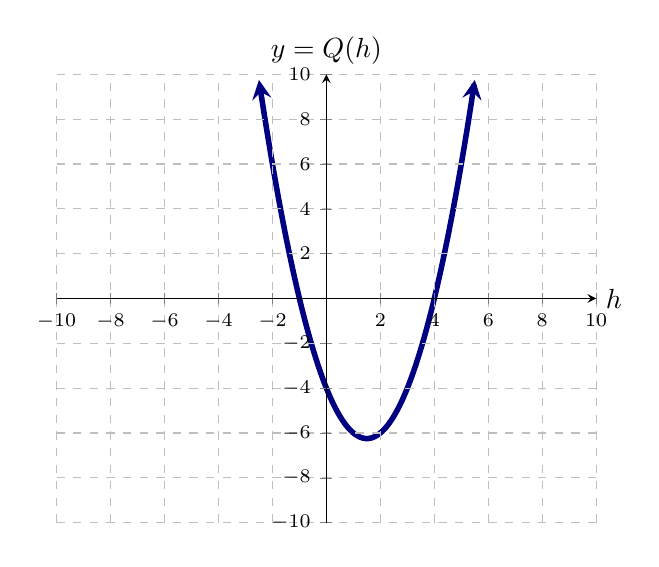
\begin{tikzpicture}
  \begin{axis}[
            domain=-10:10, ymax=10, xmax=10, ymin=-10, xmin=-10,
            axis lines =center, xlabel=$h$, ylabel={$y=Q(h)$}, grid = major, grid style={dashed},
            ytick={-10,-8,-6,-4,-2,2,4,6,8,10},
            xtick={-10,-8,-6,-4,-2,2,4,6,8,10},
            yticklabels={$-10$,$-8$,$-6$,$-4$,$-2$,$2$,$4$,$6$,$8$,$10$}, 
            xticklabels={$-10$,$-8$,$-6$,$-4$,$-2$,$2$,$4$,$6$,$8$,$10$},
            ticklabel style={font=\scriptsize},
            every axis y label/.style={at=(current axis.above origin),anchor=south},
            every axis x label/.style={at=(current axis.right of origin),anchor=west},
            axis on top
          ]
          
            
      		\addplot [line width=2, penColor, smooth,samples=200,domain=(-2.5:5.5),<->] {(x+1)*(x-4)};








  \end{axis}
\end{tikzpicture}
\end{image}


We can consider $Q(h)$ as a composition.  The outside function is $Q(h) = (h+1)(h-4)$ and the inside function is the Identity function: $I(h)=h$.  

The inside function doesn't do much.  It pairs every real number with itself.  Then this is handed to $H$. Not much of a composition, but it will help us illustrate some ideas.



The natural domain of $I(h)=h$ is \textbf{$\mathbb{R}$}.  We can think of moving along the real line left to right from $-\infty$ to $\infty$.  Each real number we run across is put into $I(h)$, which just gives it right back.  Thus, the range of $I(h)$ also runs along the real line left to right from $-\infty$ to $\infty$ at the exact same speed as the domain.  The range of $I(h)$ then becomes the domain for the outside function, $Q(h)$. \\



$\blacktriangleright$  What happens when we have a different inside function? \\


Suppose $inside(h) = 5h$.


The values of $inside(h)$ still run along the real line left to right from $-\infty$ to $\infty$. What's the difference?

The difference is that the identity function ran across its domain and range from $-\infty$ to $\infty$ at exactly the same rate - because the input and out were equal - it was the identity function.


Now the range is running through the real line left to right from $-\infty$ to $\infty$ - five times as fast as the domain. A little movement in the domain results in a lot of movement in the range and this range is the domain for $Q(h)$.






\begin{paradox}

When we graph a composition function, $Outside \circ Inside$, on the Cartesian plane, we have to picture a two-step process, where the switch is hidden from view.  

Normally, when we graph one function, the horizontal axis represents the domain of the function and the vertical axis represents the range of the same function.

With a composition, the horizontal axis represents the domain of the $Inside$ function and the vertical axis represents the range of the $Outside$ function.  There is a hidden switch occurring from the range of the $Inside$ to the domain of the $Outside$.

\end{paradox}

As we run across the horizontal axis, these values are going into $inside(h) = 5h$.  The output values, $5h$ are the new (hidden) horizontal axis for the inputs (domain) into $Outside(h) = Q(h)$.

As you run across the $h$-axis, those values are not going into $Q$.  $5$ times those values are going into $Q$.





\begin{observation}






$Q(h)$ has a zero at $-1$ and at $4$.  These are separated by a distance of $5$. The domain of $Q(h)$ needs to run this distance of $5$ from $-1$ to $4$ to get from one zero to the other.


That means the range of $inside(h)$ must run from  $-1$ to $4$ to get from one zero to the other, because the range of $inside(h)$ is the domain of $Q(h)$.

Which brings us to the domain of $inside(h)$, for our composition. 

The domain of $inside(h)$ doesn't need to run that distance of $5$, because its movement gets amplified by a factor of $5$ through the $inside$ function.  The domain of $inside$ needs to run from $-\frac{1}{5}$ to $\frac{4}{5}$ - a distance of $1$




\begin{itemize}
\item $(Q \circ inside)\left(-\frac{1}{5}\right) = Q\left(inside\left(-\frac{1}{5}\right)\right) = Q(-1) = 0$
\item $(Q \circ inside)\left(\frac{4}{5}\right) = Q\left(inside\left(\frac{4}{5}\right)\right) = Q(4) = 0$
\end{itemize}


In the $(Q \circ inside)$ function, the zeros are at $-\frac{1}{5}$ and $\frac{4}{5}$.  They are a distance of $1$ apart.  The $inside$ function has squeezed them closer together by making its range run faster than its domain - and that range became a new faster running domain for $Q$.




\end{observation}













\begin{image}
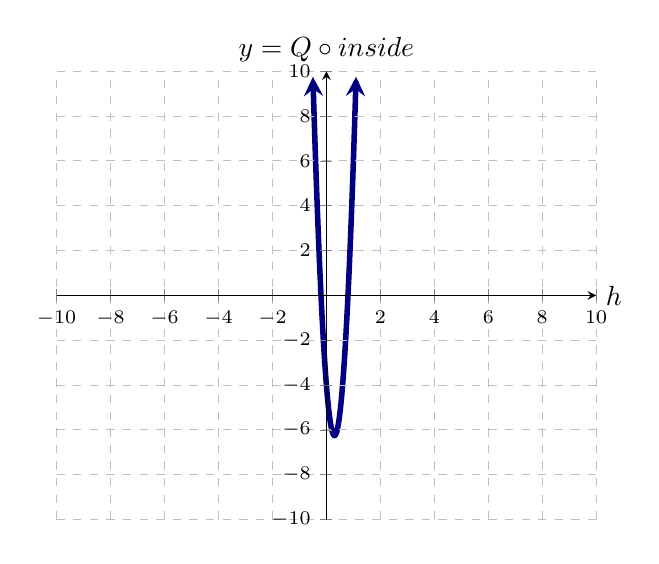
\begin{tikzpicture}
  \begin{axis}[
            domain=-10:10, ymax=10, xmax=10, ymin=-10, xmin=-10,
            axis lines =center, xlabel=$h$, ylabel={$y=Q \circ inside$}, grid = major, grid style={dashed},
            ytick={-10,-8,-6,-4,-2,2,4,6,8,10},
            xtick={-10,-8,-6,-4,-2,2,4,6,8,10},
            yticklabels={$-10$,$-8$,$-6$,$-4$,$-2$,$2$,$4$,$6$,$8$,$10$}, 
            xticklabels={$-10$,$-8$,$-6$,$-4$,$-2$,$2$,$4$,$6$,$8$,$10$},
            ticklabel style={font=\scriptsize},
            every axis y label/.style={at=(current axis.above origin),anchor=south},
            every axis x label/.style={at=(current axis.right of origin),anchor=west},
            axis on top
          ]
          
            
      		\addplot [line width=2, penColor, smooth,samples=200,domain=(-0.5:1.1),<->] {(5*x+1)*(5*x-4)};








  \end{axis}
\end{tikzpicture}
\end{image}




All of the $Q$ values are still there.  The output of $Q \circ inside$ are the same values of $Q$.  They are just connected to faster running domain values then before.








\begin{example}  Slower


How do we slow down $Q$? \\

We feed $Q$ its domain slower. \\



Let $L(x) = \frac{x}{2}$.  $L$ takes in real numbers and gives half their value to $Q$.  If we feed these into $Q$, then $Q$ will think it is only getting half the value that we see on the horizontal axis.



Graph of $y = (Q \circ L)(x) = Q(L(x))$




\begin{image}
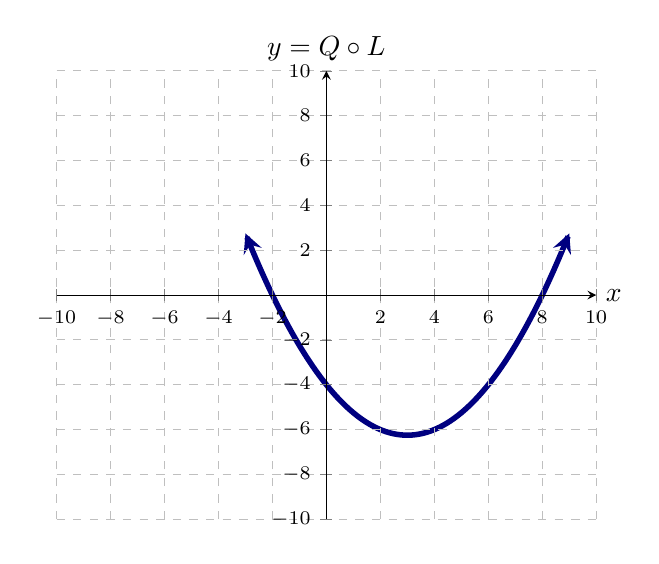
\begin{tikzpicture}
  \begin{axis}[
            domain=-10:10, ymax=10, xmax=10, ymin=-10, xmin=-10,
            axis lines =center, xlabel=$x$, ylabel={$y=Q \circ L$}, grid = major, grid style={dashed},
            ytick={-10,-8,-6,-4,-2,2,4,6,8,10},
            xtick={-10,-8,-6,-4,-2,2,4,6,8,10},
            yticklabels={$-10$,$-8$,$-6$,$-4$,$-2$,$2$,$4$,$6$,$8$,$10$}, 
            xticklabels={$-10$,$-8$,$-6$,$-4$,$-2$,$2$,$4$,$6$,$8$,$10$},
            ticklabel style={font=\scriptsize},
            every axis y label/.style={at=(current axis.above origin),anchor=south},
            every axis x label/.style={at=(current axis.right of origin),anchor=west},
            axis on top
          ]
          
            
          \addplot [line width=2, penColor, smooth,samples=200,domain=(-3:9),<->] {(0.5*x+1)*(0.5*x-4)};








  \end{axis}
\end{tikzpicture}
\end{image}


The graph is wider, because $Q$ thinks it is getting half the value as the $x$-axis. 




\end{example}

The vertical heights haven't changed. The formula $Q(L(x))$ stills say that the values of $Q$ will be the outputs - just not at the same places.



The minimum value of $Q(h) = (h+1)(h-4)$ is $-\frac{25}{4} = -6.25$, which occurs at $\frac{3}{2}$. \\

The minimum value of $Q \circ L$ is still $-\frac{25}{4} = 6.25$. It now occurs at $\frac{3}{2} \cdot 2 = 3$.  It occurs at $3$, so that when $L$ multiplies by $\frac{1}{2}$, the number $\frac{3}{2}$ is fed into $Q$. \\


The vertex on $y = Q$ was $\left (\frac{3}{2}, -\frac{25}{4} \right)$. This has moved to $\left (3, -\frac{25}{4} \right)$ for $y = Q \circ L$.


The zeros for $Q$ are $-1$ and $4$.  These move to $-2$ and $8$ for $Q \circ L$.  




\begin{question}


Let $R(t) = (t+7)(t-2)(t-5)$ \\

Let $L(x) = 3x$ \\


$-7$ is a zero of $R$.  The corresponding zero of $R \circ L$ is $\answer{\frac{-7}{3}}$.

$2$ is a zero of $R$.  The corresponding zero of $R \circ L$ is $\answer{\frac{2}{3}}$.

$5$ is a zero of $R$.  The corresponding zero of $R \circ L$ is $\answer{\frac{5}{3}}$.


\end{question}












\begin{question}


Let $p(x) = (x+6)(x+2)(x+4)$ \\

Let $L(t) = \frac{t}{5}$ \\


$-6$ is a zero of $p$.  The corresponding zero of $p \circ L$ is $\answer{-30}$.

$-2$ is a zero of $p$.  The corresponding zero of $p \circ L$ is $\answer{-10}$.

$-4$ is a zero of $p$.  The corresponding zero of $p \circ L$ is $\answer{-20}$.


\end{question}










\begin{question}


Let $T(y) = \sqrt{y-10}$ \\

Let $L(k) = -2k$ \\


The domain of $T$ is $[10, \infty)$.  The domain of $T \circ L$ is $\left( -\infty, \answer{-5} \right]$.


\end{question}
















\begin{center}
\textbf{\textcolor{green!50!black}{ooooo-=-=-=-ooOoo-=-=-=-ooooo}} \\

more examples can be found by following this link\\ \link[More Examples of Transforming the Inside]{https://ximera.osu.edu/csccmathematics/precalculus1/precalculus1/transformationsInside/examples/exampleList}

\end{center}

\end{document}
